\chapter{Introduction}
\label{chapter:introduction}

Increasingly heterogeneous hardware, including CPUs, GPUs, and accelerators, often relies on shared-memory interfaces to access and exchange data. However, different architectures can allow different shared-memory behaviors because of different hardware designs. As a result, the same concurrent program can behave differently across hardware~\cite{sewell2010x86tso,10.1145/3458926ArmedCat,DennisPhdThesis}. These architecture-specific shared-memory behaviors are described by memory consistency models. A memory consistency model specifies which memory values a thread is allowed to observe during execution~\cite{lam1675439}.

Let us first consider a concrete example called \texttt{Store-Buffering}, shown in Figure~\ref{fig:litmus-test}. This example is a litmus test, a small concurrent program used to expose and compare weak-memory behaviors~\cite{10.1145/2627752,sewell2010x86tso}. It shows how unexpected concurrent behavior can occur on the x86 architecture. The program initializes \texttt{X} and \texttt{Y} to 0. Each thread writes 1 to one variable and then reads the other variable. From a simple programmer's perspective, it may seem impossible for both \texttt{a} and \texttt{b} to be 0, because the read instructions appear after the write instructions in program order. Therefore, one might expect that at least one of the write instructions should become visible before the reads occur, so at least one read should observe 1. However, if we run this program thousands of times, we may find that both \texttt{a} and \texttt{b} can be 0. In this result, both reads still observe the old initial values. This behavior is unexpected.

\begin{figure}[h]
\centering
\[
\begin{array}{c}
\text{Initially: } X = 0,\; Y = 0
\end{array}
\qquad
\begin{array}{c|c}
\text{Thread 0} & \text{Thread 1} \\
\hline
X := 1          & Y := 1 \\
a := Y          & b := X
\end{array}
\]
\caption{Store-Buffering litmus test}
\label{fig:litmus-test}
\end{figure}

The x86-TSO programmer's model in Figure~\ref{fig:tso-mem} explains why we can observe this unexpected result~\cite{sewell2010x86tso}. In each thread, x86 has a store buffer. When a processor writes a value to memory, it first places the value in the store buffer. Later, the store buffer writes this value to shared memory. Now let us return to the \texttt{Store-Buffering} program in Figure~\ref{fig:litmus-test}. Thread 0 and Thread 1 first place their new values in their store buffers. At this point, the updated values of \texttt{X} and \texttt{Y} are still in the store buffers, not in shared memory. Then, Thread 0 and Thread 1 read from shared memory. Because shared memory still contains the old values, both threads read the old values. As a result, both \texttt{a} and \texttt{b} can be 0.

\begin{figure}[htbp]
  \centering
  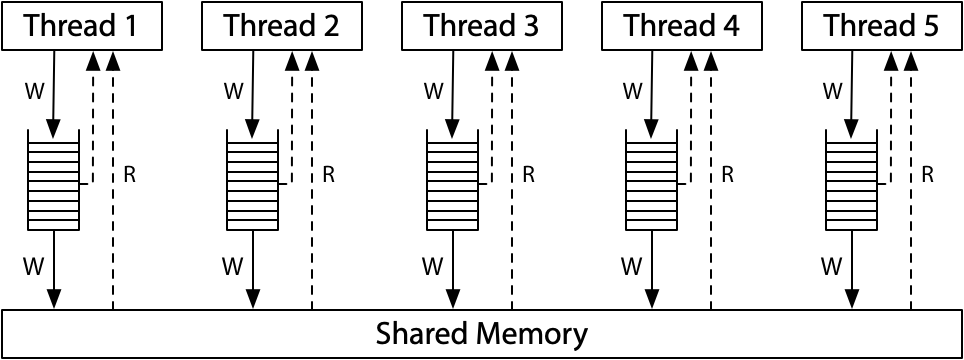
\includegraphics[width=\textwidth]{thesis/figures/mem-tso@2x.png}
  \caption{The x86 memory architecture diagram.}
  \label{fig:tso-mem}
\end{figure}

This unexpected behavior may seem unlikely to introduce bugs because it is subtle: we may need to run the same program thousands of times before observing the unexpected result. However, code with a similar structure can be used for synchronization between threads. For example, low-level systems code often needs to coordinate access to shared data across multiple cores. A simplified flag-based synchronization pattern is shown in Figure~\ref{fig:flag-sync}. In this example, each thread has a loop that checks a flag. If another thread is accessing the data, the current thread waits in the loop. This style of flag-based synchronization is related to algorithms such as Dekker's algorithm~\cite{dijkstra1965cooperating}.

\begin{figure}[h]
\centering
\[
\begin{array}{c}
\text{Initially: } \texttt{flag1 = false},\; \texttt{flag2 = false}
\\[0.5em]
\begin{array}{c|c}
\text{Thread 1} & \text{Thread 2} \\
\hline
\begin{array}{l}
\texttt{flag1 := true} \\
\texttt{while flag2 == true do} \\
\quad \texttt{wait} \\
\texttt{access\_data()} \\
\texttt{flag1 := false}
\end{array}
&
\begin{array}{l}
\texttt{flag2 := true} \\
\texttt{while flag1 == true do} \\
\quad \texttt{wait} \\
\texttt{access\_data()} \\
\texttt{flag2 := false}
\end{array}
\end{array}
\end{array}
\]
\caption{Flag-based synchronization example}
\label{fig:flag-sync}
\end{figure}

The problem is that, when the written flag values are still in the store buffers in the x86 architecture, each processor may think that the other thread is not accessing the data. As a result, both threads may enter the critical section at the same time. This breaks the intended synchronization and can introduce a data race. Data races can cause unexpected behavior, such as corrupted data, inconsistent results, or crashes~\cite{batty2011mathematizing,alglave2018frightening}. Therefore, even if the unexpected result is hard to observe in one run of one program, the problem still matters because similar synchronization patterns are widely used in low-level software.

This unexpected behavior is not specific to x86. As we have seen, it is related to the store-buffer design in the architecture. Other architectures, such as ARM and RISC-V, can allow even more subtle behaviors in their shared-memory designs~\cite{10.1145/3458926ArmedCat,riscv-spec,DennisPhdThesis}. Thus, even if we have exactly the same program, compile it, and run it on different architectures, we may observe different results. These nondeterministic behaviors can cause many subtle problems for programmers, compiler writers, and verification tools. Therefore, we need a way to reason about shared-memory behaviors across different architectures.

One intuitive way to study memory consistency models is to run many different litmus tests many times and observe their possible results. Litmus tests are useful because they can expose subtle behaviors allowed by a memory system~\cite{10.1145/2627752}. However, testing alone is not enough for reasoning about memory consistency models, because there are infinitely many ways to write concurrent programs. We cannot enumerate all possible concurrent programs and run them on hardware to obtain a general description of the memory system.

Instead of considering only concrete litmus tests, we can represent program executions in a more general way. In axiomatic memory models, executions are commonly represented using events and relations between events~\cite{10.1145/2627752,10.1145/3458926ArmedCat}. In concurrent programming, we often care about the ordering relationships between instructions: which instructions are ordered before others, which writes are observed by which reads, and how writes to the same memory location are ordered. These relationships can be represented by arrows. If one instruction points to another, the arrow represents a relation between the two instructions. These instructions and arrows together form an \texttt{execution graph}.

One possible execution graph is called a \texttt{candidate execution}: it represents one possible assignment of events and relations for a litmus-test outcome before a memory model decides whether that outcome is allowed~\cite{catManualSyntax11,10.1145/2627752}. For example, when the \texttt{Store-Buffering} program in Figure~\ref{fig:litmus-test} produces the result \texttt{a = 0} and \texttt{b = 0}, it can be represented as the execution graph in Figure~\ref{fig:litmus-execution-0-0}. In the graph, \texttt{W(X)=v} denotes a write of value \texttt{v} to location \texttt{X}, and \texttt{R(Y)=v} denotes a read from \texttt{Y} that returns value \texttt{v}.

\begin{figure}[htbp]
\centering
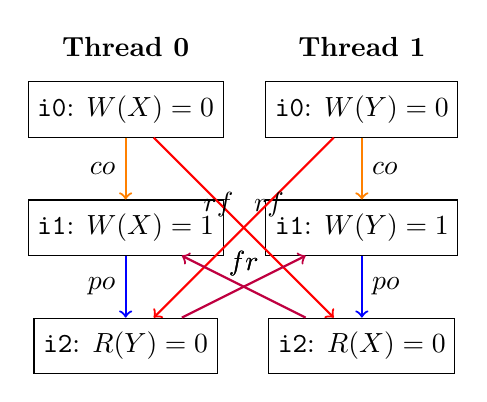
\begin{tikzpicture}[
    node distance=1cm,
    event/.style={draw, rectangle, minimum width=1.8cm, minimum height=0.7cm},
    po/.style={->, thick, blue},
    rf/.style={->, thick, red},
    co/.style={->, thick, orange},
    fr/.style={->, thick, purple}
]

% Thread labels
\node[draw=none] (t0label) at (-1.5,0.8) {\textbf{Thread 0}};
\node[draw=none] (t1label) at ( 1.5,0.8) {\textbf{Thread 1}};

% Initial writes
\node[event] (initX) at (-1.5,0) {\texttt{i0}: $W(X)=0$};
\node[event] (initY) at ( 1.5,0) {\texttt{i0}: $W(Y)=0$};

% Thread 0 events
\node[event] (wx1) at (-1.5,-1.5) {\texttt{i1}: $W(X)=1$};
\node[event] (ry0) at (-1.5,-3)   {\texttt{i2}: $R(Y)=0$};

% Thread 1 events
\node[event] (wy1) at ( 1.5,-1.5) {\texttt{i1}: $W(Y)=1$};
\node[event] (rx0) at ( 1.5,-3)   {\texttt{i2}: $R(X)=0$};

% Program order
\draw[po] (wx1) -- node[left, black] {$po$} (ry0);
\draw[po] (wy1) -- node[right, black] {$po$} (rx0);

% Reads-from
\draw[rf] (initY) -- node[above right, black] {$rf$} (ry0);
\draw[rf] (initX) -- node[above left, black] {$rf$} (rx0);

% Coherence order
\draw[co] (initX) -- node[left, black] {$co$} (wx1);
\draw[co] (initY) -- node[right, black] {$co$} (wy1);

% From-read
\draw[fr] (ry0) -- node[above, black] {$fr$} (wy1);
\draw[fr] (rx0) -- node[above, black] {$fr$} (wx1);

\end{tikzpicture}
\caption{Candidate execution for the outcome $R(Y)=0$ and $R(X)=0$. Blue arrows show program order (\textit{po}), red arrows show reads-from (\textit{rf}), orange arrows show coherence order (\textit{co}), and purple arrows show from-read (\textit{fr}).}
\label{fig:litmus-execution-0-0}
\end{figure}

The candidate execution in Figure~\ref{fig:litmus-execution-0-0} has four kinds of arrows:

(1) The blue arrows show program order (\textit{po}), which indicates the order of instructions in each thread. For example, in each thread, there is a \textit{po} edge from \texttt{i1} to \texttt{i2}. This means that \texttt{i1} is before \texttt{i2} in program order.

(2) The orange arrows show coherence order (\textit{co}), which orders writes to the same memory location. For example, the write \texttt{W(X)=1} is later than the initial write \texttt{W(X)=0} in the coherence order for location \texttt{X}. Similarly, the write \texttt{W(Y)=1} is later than the initial write \texttt{W(Y)=0} in the coherence order for location \texttt{Y}.

(3) The red arrows show reads-from (\textit{rf}), which indicates which write a read observes. In this candidate execution, both reads return the initial values. For example, the read \texttt{R(Y)=0} in Thread 0 reads from the initial write \texttt{W(Y)=0}, and the read \texttt{R(X)=0} in Thread 1 reads from the initial write \texttt{W(X)=0}. Therefore, both reads observe the initial writes.

(4) The purple arrows show from-read (\textit{fr}), which relates a read to a later write that overwrites the value read. For example, \texttt{R(Y)=0} in Thread 0 reads the initial value of \texttt{Y}, but this value is later overwritten by \texttt{W(Y)=1} in Thread 1. Therefore, there is an \textit{fr} edge from \texttt{R(Y)=0} to \texttt{W(Y)=1}. Similarly, \texttt{R(X)=0} in Thread 1 reads the initial value of \texttt{X}, but this value is later overwritten by \texttt{W(X)=1} in Thread 0. Therefore, there is an \textit{fr} edge from \texttt{R(X)=0} to \texttt{W(X)=1}.

Execution graphs give us a systematic way to describe possible program behaviors. Once program behaviors are represented as graphs, memory consistency models can be expressed as rules over these graphs. For example, some memory consistency models forbid candidate executions when certain combinations of relations contain a cycle. In Figure~\ref{fig:litmus-execution-0-0}, if we follow the \textit{po} and \textit{fr} edges, we obtain a cycle:
\[
W(X)=1 \xrightarrow{po} R(Y)=0 \xrightarrow{fr} W(Y)=1 \xrightarrow{po} R(X)=0 \xrightarrow{fr} W(X)=1.
\]
A stricter memory consistency model may forbid this candidate execution because of this cycle. However, weaker memory consistency models, such as x86-TSO, do not necessarily forbid this behavior in the same way. This is why the same candidate execution may be allowed by one memory consistency model but forbidden by another.

This observation connects memory consistency models to mathematical reasoning. The arrows in an execution graph can be viewed as binary relations between events. A binary relation describes a connection between two things, such as two instructions in an execution. Therefore, many questions about memory consistency models can be treated as mathematical questions about binary relations, such as whether a relation is acyclic or whether one set of allowed executions is included in another. We will explain binary relations in detail in Chapter~\ref{chapter:Background}.

Before we go further, we explain why memory consistency models are important and why we want to use formal methods to reason about them.

\subsubsection{Why Are Memory Consistency Models Important?}

A memory consistency model describes the shared-memory behaviors allowed by an architecture~\cite{lam1675439,sewell2010x86tso}. Therefore, it can serve as a useful intermediate specification between programs and hardware. This is important because each architecture may have its own way to interact with shared memory. When different architectures are used together, or when software is moved from one architecture to another, we need to understand how their memory behaviors relate to each other. Many problems in heterogeneous systems can therefore be understood as problems about memory consistency models.

One important problem is comparing different memory consistency models. A memory consistency model is stronger if it allows fewer behaviors. For example, if a new architecture specification fixes a mistake in an older specification, we may want to prove that the new memory consistency model is stronger than the previous one. This would show that the new model forbids some incorrect behaviors that were allowed by the old model.

Another important problem is the correctness of heterogeneous hardware. Different devices may need to be connected at the hardware level. This requires, among other things, combining each intra-device coherence protocol with a global inter-device coherence protocol, such as ARM CHI~\cite{arm2021chi} or CXL~\cite{cxl2022}. However, this combination can be done incorrectly. If the joint model is too strong, it may hurt performance. Worse, if the joint model is too weak, it may break correctness. Therefore, having a clear intermediate specification is necessary to ensure that the hardware is designed correctly.

Memory consistency models are also useful for reasoning about binary translation and compiler correctness~\cite{10.1145/2676726.2676995,DennisPhdThesis}. For example, when translating x86 binaries to RISC-V binaries at the machine-code level, we need to verify whether the translation is safe. One way to state this requirement is to compare the memory behaviors of the source and target programs. If every behavior of the translated RISC-V program is allowed by the original x86 program, then the translation preserves the memory behavior of the source program.

Memory consistency models are also important for interoperability between different layers of a system. For example, a program may be written in a language such as C, compiled into machine code, and executed on hardware that follows an architectural memory consistency model~\cite{batty2011mathematizing,podkopaev2019bridging}. In systems such as the Linux kernel, we may also need to reason about the relationship between the programming-language memory consistency model, the Linux kernel memory consistency model, and the hardware memory consistency model~\cite{alglave2018frightening}. To reason about the correctness of the whole system, we need formal ways to compare and combine these models.

\subsubsection{Why Use Formal Methods?}

As described above, testing is useful for detecting the behaviors of a specific concurrent program by running it many times and observing its results. However, testing itself cannot cover all possible program behaviors. It also cannot provide a general way to describe these behaviors or reason about them across different architectures.

Formal methods address this limitation by describing program executions using mathematical structures, such as binary relations, and by imposing axioms on these structures~\cite{10.1145/2627752,10.1145/3458926ArmedCat}. This gives us a systematic way to reason about memory behaviors. Binary relations can be studied mathematically, and many existing theorems about relations can be used to reason about execution graphs and memory consistency models~\cite{rosen2012discrete}.

Formal memory consistency models are useful because they allow us to reason about architectures in a general way. They are not only used to explain why a specific behavior can happen on one architecture, but also to compare the behaviors allowed by different architectures. This is important because modern systems often involve multiple architectures, and the same concurrent program may behave differently on different hardware. Therefore, we need tools that can support both concrete reasoning about one architecture and general comparison between architectures.

Both testing and formal methods are useful for studying weak memory consistency models. Testing helps us observe concrete behaviors, while formal methods help us describe and reason about the general space of possible behaviors. Therefore, a useful tool should support both concrete examples, such as litmus tests, and general mathematical reasoning about memory consistency models.

\subsubsection{Contributions}

In practice, many memory consistency models are written in Cat, a domain-specific language for specifying memory consistency models~\cite{10.1145/2627752,catOnlineDocHerd,catManualSyntax11}. Cat describes relations between events in a candidate execution, such as program order, reads-from, coherence order, and from-read. It also uses axioms, such as acyclicity constraints, to decide whether a candidate execution is allowed or forbidden by a memory consistency model.

Cat is therefore a useful starting point for mechanized reasoning. Instead of rewriting memory consistency models from scratch in a proof assistant, we can reuse existing Cat specifications. However, Cat specifications themselves are not machine-checked proofs. They describe the allowed executions of a memory consistency model, but they do not by themselves provide a proof infrastructure for proving general properties about memory consistency models, such as model inclusion, preservation across updates, or correctness of translations between architectures.

To address this problem, we use interactive theorem proving. Lean 4 is an interactive theorem prover (ITP), which allows us to write mathematical definitions and proofs that are checked by a machine~\cite{deMoura2021lean4}. Mechanization requires additional work, because definitions and proofs must be encoded in the proof assistant. However, it also provides important benefits: it reduces mistakes, makes definitions and lemmas reusable, and makes proofs easier to maintain when memory consistency models change.

In this work, we use Lean 4 and Mathlib. Lean 4 allows us to mechanize memory consistency model definitions and proofs, so that the proof assistant can check the correctness of our reasoning. Lean 4 also provides a powerful metaprogramming framework~\cite{10.1145/3110278Lean4Meta}, which is important for LeanCat because LeanCat automatically generates Lean definitions from Cat specifications. This reduces the amount of manual encoding required and helps keep the mechanized definitions consistent with the original memory consistency model specifications. Mathlib provides a rich library of reusable mathematical definitions and lemmas, giving us a strong foundation for reasoning about relations, orders, sets, and other mathematical structures used in memory consistency models~\cite{mathlib2020}.

We present LeanCat, a proof infrastructure that connects these two sides: it reuses Cat specifications as input and turns them into Lean 4 definitions for mechanized proofs. As discussed above, many questions about memory consistency models can be converted into questions about binary relations, such as whether a relation is acyclic or whether one memory consistency model allows fewer behaviors than another. These questions can be stated mathematically, and in principle, they can be proved by pen-and-paper reasoning. However, pen-and-paper proofs are difficult to check, easy to get wrong, and hard to maintain when memory consistency models evolve.

LeanCat translates memory consistency models written in Cat into binary relations in Lean 4. LeanCat has several advantages. First, it improves reuse: existing Cat memory consistency models can be translated into Lean 4 definitions instead of being rewritten from scratch. Second, it improves consistency: when a memory consistency model changes, such as an update to the ARMv8 memory consistency model, LeanCat can regenerate the Lean definitions and help check the related properties again. Third, it supports both concrete and general reasoning: it can check whether a specific litmus test is allowed under a particular architecture, and it can also be used to prove more general properties between different architectures. Finally, LeanCat is user-friendly: it provides interfaces that allow users to inspect the execution graph of a litmus test and understand why a behavior is allowed or forbidden.
